%
% IAT 267: Introduction to Technological Systems - A Course Overview
% Section: Arduino
%
% Author: Jeffrey Leung
%

\section{Arduino}
	\label{sec:arduino}
\subsection{Setup}
	\label{subsec:arduino:setup}
\begin{easylist}

	& Plug the Arduino into the computer
	& Open the Arduino IDE
	& Select the correct board and serial port
	& Verify and upload the program to the Arduino

\end{easylist}
\subsection{Physical Configuration}
	\label{subsec:arduino:physical-configuration}
\begin{easylist}

	& Figure~\ref{fig:arduino-uno-diagram} shows the layout of an Arduino Uno. \\
	The top pins are for digital input and output (and analog output, through \hyperref[sec:actuators]{PWM}). \\
	The bottom centre pins are for the standard power source and grounding. \\
	The bottom right pins are for analog input.

	\begin{figure}[!htb]
		\centering
		\href
		{https://www.element14.com/community/groups/arduino/blog/2014/12/17/rgb-led-shield-diagrams-for-documentation-purposes}
		{
			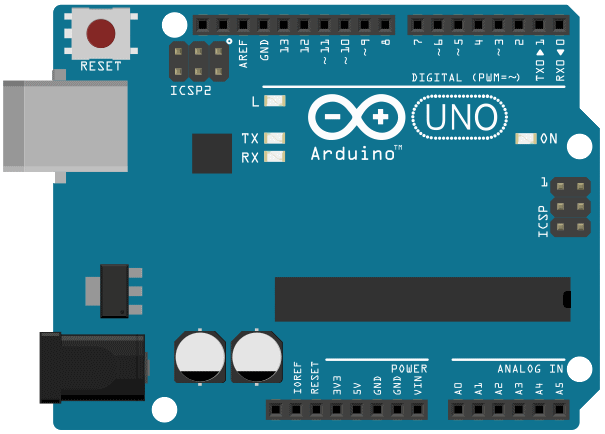
\includegraphics[scale=.5]{arduino-uno-diagram}
		}
		\caption{Arduino Uno Diagram}
		\label{fig:arduino-uno-diagram}
	\end{figure}

	& Uses an Atmel megaAVR \hyperref[subsubsec:electricity-and-circuit-design:circuits:components]{microcontroller}

	& Plugging in the USB cable provides power to the circuit

	& Power terminals:
		&& Positive: 5V
		&& Negative: GND (ground)

	& Switch:
		&& If the prongs are lined up vertically, the left prongs (top and bottom) are connected and the right prongs (top and bottom) are connected. When the button is pressed, the connection between the left pair and the right pair is bridged.
			&&& See figure~\ref{fig:arduino-switch} for an illustration of the prongs

			\begin{figure}[!htb]
				\centering
				\href
				{https://www.sparkfun.com/products/9190}
				{
					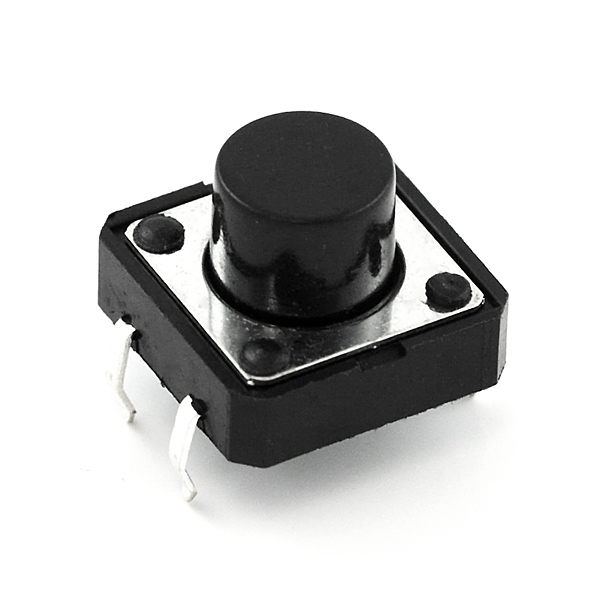
\includegraphics[scale=.3]{arduino-switch}
				}
				\caption{Momentary Pushbutton Switch. Activating the button bridges the two visible prongs.}
				\label{fig:arduino-switch}
			\end{figure}

	& Digital pin 13 has a built-in resistor

\end{easylist}
\subsubsection{Input/Output}
	\label{subsec:arduino:input-output}
\begin{easylist}

	& Digital input/output: Digital pins
		&& Can accept \textbf{HIGH} (5V) or \textbf{LOW} (0V)

	& Analog input: Analog pins
		&& Reads a value from 0 to 1023, proportional to the input voltage (0V to 5V)
		&& Uses an \hyperref[subsubsec:electricity-and-circuit-design:circuits:components]{analog-to-digital converter} in the Atmel megaAVR microcontroller in the Arduino
			&&& 6-channel
			&&& 10-bit resolution (1024 values)
		&& Requires a \hyperref[subsubsec:electricity-and-circuit-design:circuits:types-of-circuits]{voltage divider}

	& Analog output: Digital pins with the \textbf{\~{}} (tilde)
		&& Takes a value between 0 and 255, proportional to the amount of time that the voltage output is activated
			&&& Rapidly alternates between 0V and 5V
		&& All microcontrollers can only output a digital voltage, not an analog voltage
			&&& Uses \hyperref[sec:actuators]{pulse-width modulation} to simulate analog output

	& \hyperref[subsec:technological-systems:interaction]{Serial communication:}
		&& 8-bit communication
		&& \textbf{Serial.begin()} sets the data rate
		&& Digital pin 0 receives data (labeled RX)
		&& Digital pin 1 transmits data (labeled TX)
		&& \href{http://arduino.cc/en/Reference/Serial}{Arduino serial library}
		&& Only one program can receive serial input at a given time (e.g. Processing and the Arduino serial monitor cannot receive serial input at the same time)

\end{easylist}
\subsection{Programming}
	\label{subsec:arduino:programming}
\begin{easylist}

	& Arduino programming language:
	 	&& Set of C and C++ functions
		&& Compiled with \emph{avr-g++}
		&& Open source

	& \emph{Sketch:} Program written for an Arduino

	& \lstinline{void setup()}:
		&& Custom-defined function
		&& Run once before the other code
	& \lstinline{void loop()}:
		&& Custom-defined function
		&& Run continually
	& \lstinline{void serialEvent()}:
		&& Custom-defined function
		&& Executed after each iteration of the \lstinline{void loop()} function

	& Arduino libraries:
		&& \href{https://www.arduino.cc/en/Reference/Serial}{Serial}
		&& \href{https://www.arduino.cc/en/Reference/Servo}{Servo}
		&& \href{https://www.arduino.cc/en/Reference/softwareSerial}{SoftwareSerial}

\end{easylist}
\clearpage
